
%part 2
\subsection{Annexe A : Diagramme d'état transition de la vue d'ensemble}
\begin{figure}[!h]
\centering
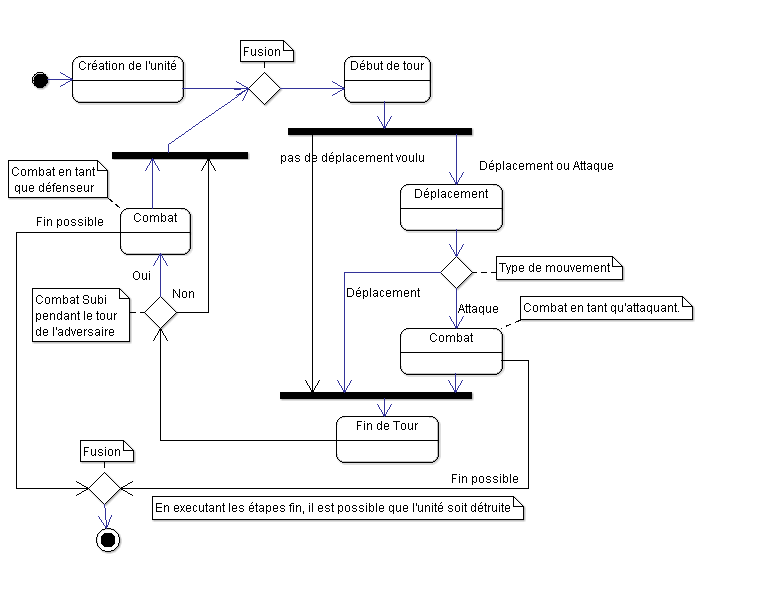
\includegraphics[scale=0.70]{img/VueDensemble.png}
\caption{Diagramme d'état transition de la vue d'ensemble}
\end{figure}
\clearpage

\subsection{Annexe B : Diagramme du déplacement d'une pièce}
\begin{figure}[!h]
\centering
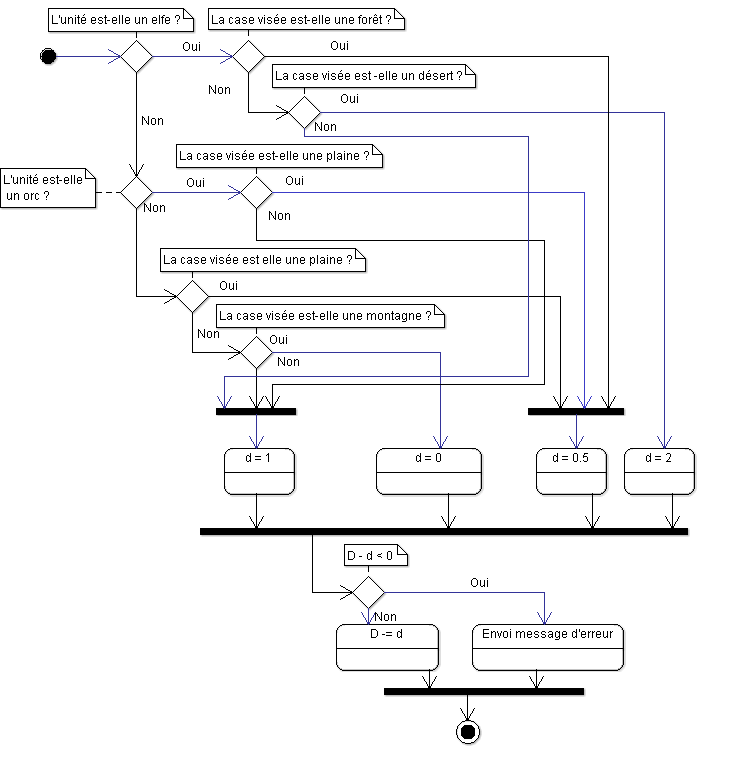
\includegraphics[scale=0.65]{img/Deplacement.png}
\caption{Diagramme d'état transition du déplcement d'une pièce}
\end{figure}
\clearpage

\subsection{Annexe C : Diagramme d'état transition du combat d'une pièce}
\begin{figure}[!h]
\centering
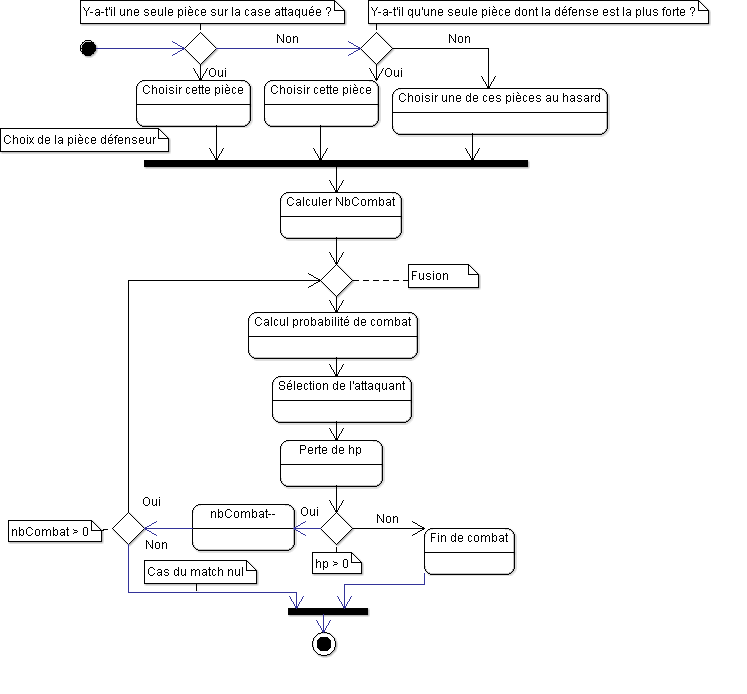
\includegraphics[scale=0.75]{img/Combat.png}
\caption{Diagramme d'état transition du combat d'une pièce}
\end{figure}
\clearpage

\subsection{Annexe D : Diagramme d'état transition des cas de fin de combat d'une pièce}
\begin{figure}[!h]
\centering
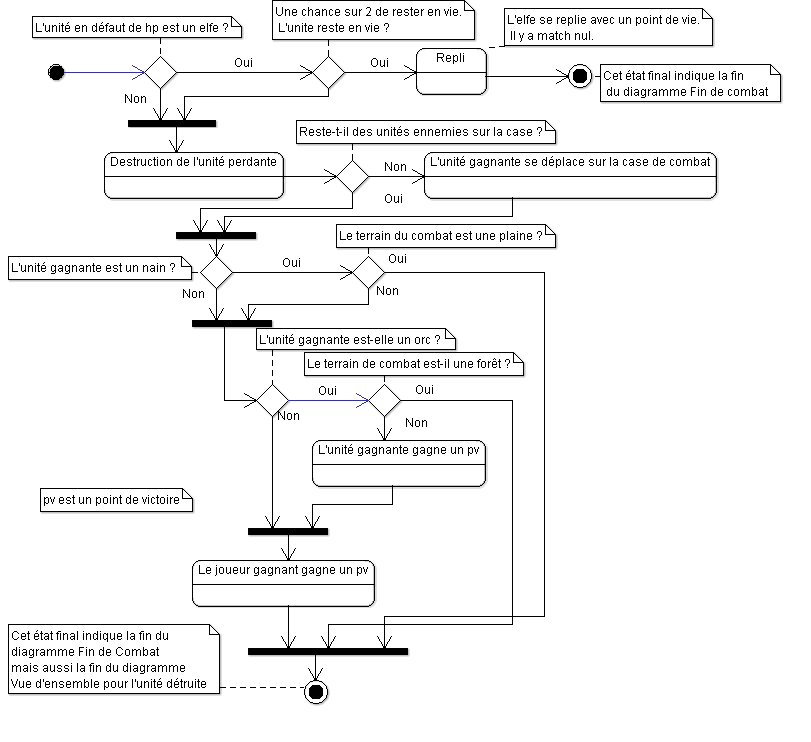
\includegraphics[scale=0.69]{img/FinDeCombat.png}
\caption{Diagramme d'état transition des cas de fin de combat d'une pièce}
\end{figure}
\clearpage

\subsection{Annexe E : Diagramme de séquence du chargement du jeu}
\begin{figure}[!h]
\centering
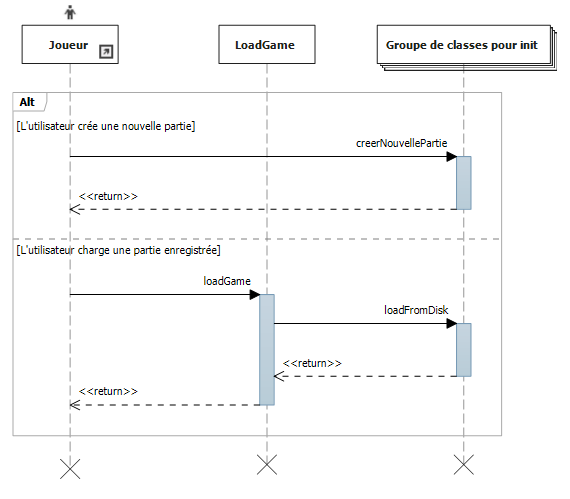
\includegraphics[width=1\textwidth]{img/LoadInitDiagram.png}
\caption{Diagramme de séquence du chargement du jeu}
\end{figure}
\clearpage

\subsection{Annexe F : Diagramme de communication des actions de l'utilisateur}
\begin{figure}[!h]
\centering
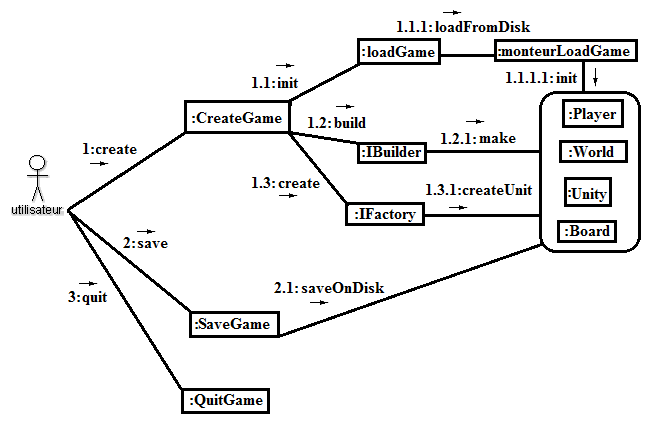
\includegraphics[width=1\textwidth]{img/com.png}
\caption{Diagramme de communication des actions de l'utilisateur}
\end{figure}
\clearpage

\subsection{Annexe G : Diagramme de séquence de l'initialisation globale}
\begin{figure}[!h]
\centering
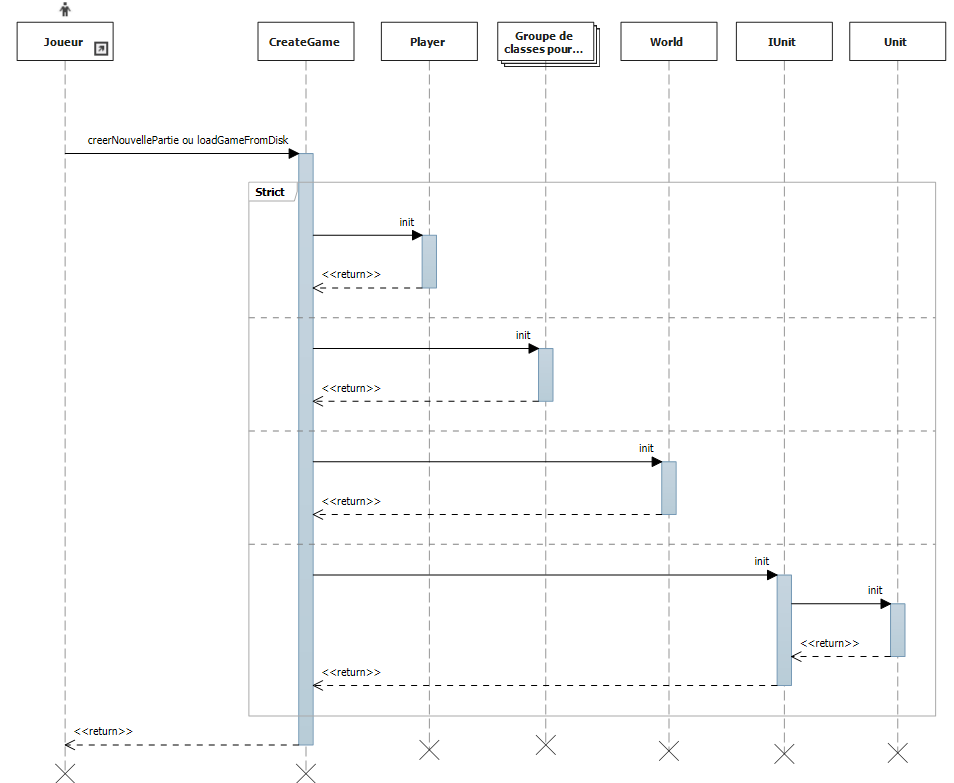
\includegraphics[width=1.1\textwidth]{img/InitAll.png}
\caption{Diagramme de séquence de l'initialisation globale}
\end{figure}
\clearpage

\subsection{Annexe H : Diagramme de séquence de l'initialisation du board}
\begin{figure}[!h]
\centering
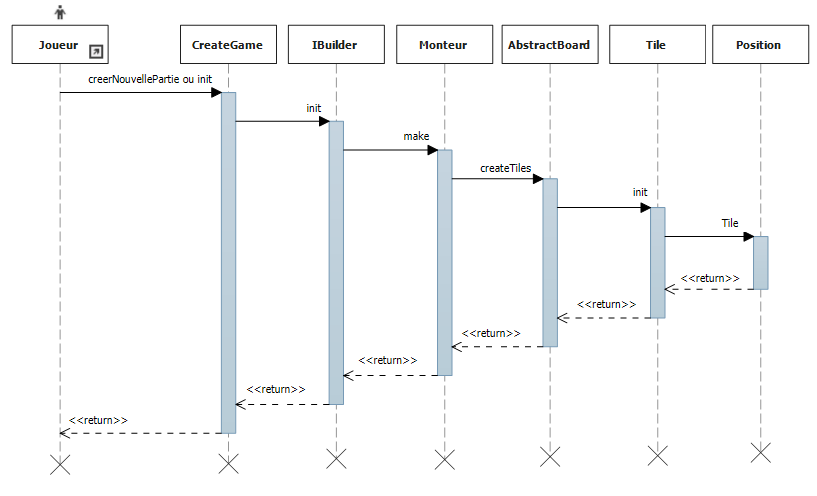
\includegraphics[width=1.1\textwidth]{img/InitBoard.png}
\caption{Diagramme de séquence de l'initialisation du board}
\end{figure}
\clearpage

\subsection{Annexe I : Diagramme de séquence des actions d'une pièce}
\begin{figure}[!h]
\centering
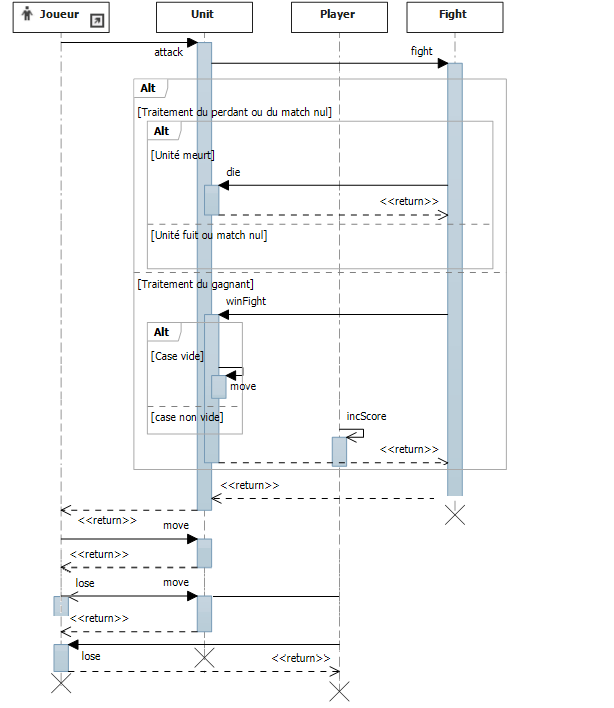
\includegraphics[width=1\textwidth]{img/Actions.png}
\caption{Diagramme de séquence des actions d'une pièce}
\end{figure}
\clearpage

\subsection{Annexe J : Diagramme de communication des actions d'une pièce}
\begin{figure}[!h]
\centering
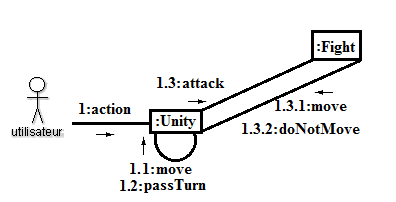
\includegraphics[width=1\textwidth]{img/comm2.png}
\caption{Diagramme de communication des actions d'une pièce}
\end{figure}
\clearpage

%part 3
\subsection{Annexe H : Diagramme de classe : structure globale}
\begin{figure}[!h]
\centering
\label{structure}
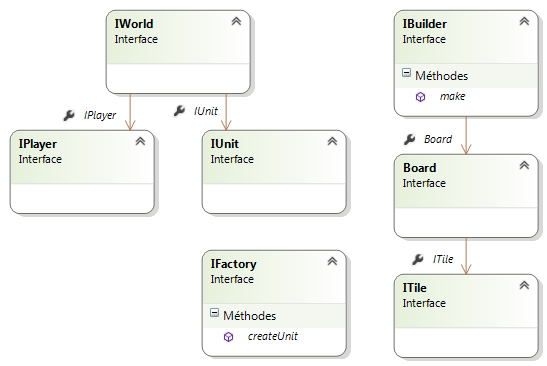
\includegraphics[width=1\textwidth]{img/Interfaces.png}
\caption{Diagramme de classe : structure globale}
\end{figure}
\clearpage


